\documentclass{article}
\usepackage[utf8]{inputenc}
\usepackage{amsmath}
\usepackage{graphicx}
\usepackage{BeginnerStyleFile}
\graphicspath{ {images/} }

\title{Reading Summary 4.1}
\author{Evan Hughes}
\date{March 2023}

\begin{document}
\maketitle
\section*{4.1 Polynomial Arithmetic and Division Algorithm}
\subsection*{Defining the Polynomial}
We must start with defining polynomials in a way that is an obvious extension of real-number coefficient polynomials.

Let $R$ be any ring. A polynomial with coefficients in $R$ is an expression of the form 

\begin{equation}
    a_0 + a_1x + a_2x^2 + \cdots + a_nx^n
\end{equation}

where $n$ is a non negative integer and $a_i \in R$.

But what is $x$? 

\subsection*{Theorem 4.1}
If $R$ is a ring, then there exists a ring T containing an element $x$
that is not in $R$ and has these properties:
\begin{enumerate}
    \item $R$ is a subring of $T$.
    \item $xa = ax$ for all $a \in R$.
    \item The set $R[x]$, read $R$ add $x$, of all elements of $T$ of from
    \begin{center}
        $a_0 + a_1x + a_2x^2 + \cdots + a_nx^n$ (where $n \geq 0$ and $a_i \in R$)
    \end{center}
    is a subring of $T$ that contains $R$.
    \item The representation of elements of $R[x]$ is unique: if
    $n \leq m$ and 
    \begin{center}
        $a_0 + a_1x + a_2x^2 + \cdots + a_nx^n = b_0 + b_1x + b_2x^2 + \cdots + b_mx^m$,
        then $a_i = b_i$ for $i = 1, 2, \cdots, n$ and $b_1 = 0_R$ if and only if $a_i=0_R$.
    \end{center}
    \item $a_0 + a_1x + a_2x^2 + \cdots + a_nx^n = 0$ if and only if $a_i = 0$ for all $i$.
\end{enumerate}

\subsection*{Proof of Theorem 4.1}
The elements of the ring $R[x]$ in Theroem 4.1 are called polynomials with coefficients in $R$.
and the elements $a_i$ are called coefficients. The special element x is sometimes called an indeterminate.
Note: 
\begin{itemize}
    \item Property 2 does not imply that the ring T is commutative, but only that the special element $x$ commutes with each element of the subring $R$.
    \item Property 5 is the special case of property 4 when each $b_i=0_r$
    \item The first expression in property 5 is not an equation to be solved for x. In this context, asking what value makes $a_0 + a_1x + \cdots + a_nx^n = 0_R$ is meaningless. This is because $x$ is a specific element of a ring, not a variable.
\end{itemize}
\subsection*{Example(from the book)}
Let $E$ be the ring of even integers. Then $4-6x+4x^3 \in E[x]$. However, the polynomial $x$ is not in $E[x]$, because it cannot be written with even coefficients.

\subsection*{Polynomial Arithmetic}
The rules for adding and multiplying polynomials follow directly from the fact that $R[x]$ is a ring.

\subsection*{Example} If $f(x) = 2+3x-4x^2$ and $g(x) = 3-2x+x^2$, then $f(x) + g(x) = 5+x-2x^2$ and $f(x)g(x) = 8-x-x^2$.

\subsection*{Theorem 4.2}
If $R$ is an integral domain and $f(x), g(x)$ are nonzero polynomials in $R[x]$, then the degree of $f(x)g(x) = $ the degree of $f(x)$ plus the degree of $g(x)$.

\subsection*{Proof of Theorem 4.2}
Suppose $f(x)=a_0+a_1x+a_2x^2+\cdots+a_nx^n$ and $g(x)=b_0 + b_1x+\cdots+b_mx^m$
with $a_n \neq 0$ and $b_m \neq 0$. so that deg$f(x) = n$ and deg$g(x) = m$. then
\begin{center}
    $f(x)g(x)=a_0b_0+(a_0b_1+a_1b_0)x+(a_2b_0+a_1b_1+a_0b_2)x^2+\cdots+a_nb_mx^{n+m}$
\end{center}
The largest exponent of $x$ that can possibly have a nonzero coefficient is
$n + m$. But $a_n b_m \neq 0_R$ because $R$ is an integral domain and $a_n \neq 0_R$ and
$b_m = 0_R$. Therefore, $f(x)g(x)$ is nonzero and deg$(f(x)g(x)) \leq n + m \leq $deg$f(x) + $deg $g(x)$

\subsection*{Corollary 4.3}
If $R$ is an integral domain, then so is $R[x]$.

\section*{Proof of Corollary 4.3}
Since $R$ is a commutative ring with identity, so is $R(x)$.
The proof of Theorem 4.2 shows that the product of nonzero polynomials
in $R(x)$ is nonzero. Therefore, $R(x)$ is an integral domain.

\subsection*{Corollary 4.4}
Let $R$ be a ring. If $f(x), g(x)$, and $f(x)g(x)$ are nonzero in $R[x]$,
then deg$[f(x)g(x)] \leq $deg$f(x) + $deg$g(x)$.

\subsection*{Corollary 4.5}
Let $R$ be an integral domain and $f(x) \in R[x]$. Then $f(x)$ is a unit in $R[x]$ if and only if $f(x)$ is a constant polynomial
that is a unit in $R$. In particular, if $F$ is a field, the units in $F[x]$ are the nonzero constants in $F$.
\vspace*{5cm}
\subsection*{The Division Algorithm in $F[x]$}
Let $F$ be a field and $f(x), g(x) \in F[x]$ with $g(x) \neq 0_F$. Then there exist unique polynomials $q(x)$ and $r(x)$ in $F[x]$ such that
\begin{center}
    $f(x) = g(x)q(x) + r(x)$ and either $r(x) = 0_F$ or deg$r(x) < $deg$g(x)$.
\end{center}

\begin{figure}
    \centering
    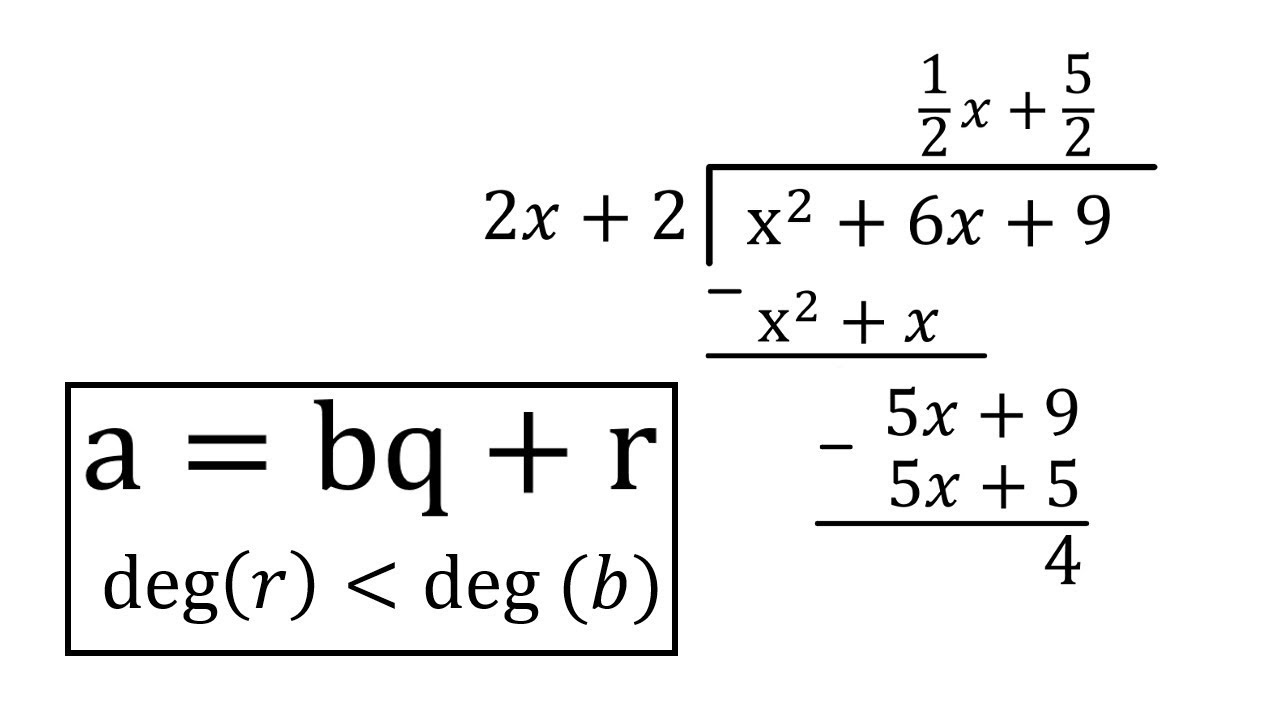
\includegraphics[width=0.5\textwidth]{divisonAlgorithm.jpg}
    \caption{Division Algorithm}
    \label{fig:division_algorithm}
\end{figure}
\end{document}